\documentclass[12pt,a4paper]{article}
\usepackage{iftex}
\ifPDFTeX
    \usepackage[utf8]{inputenc}
    \usepackage[T1]{fontenc}
    \usepackage{CJKutf8}
\else
    \usepackage[UTF8]{ctex}
\fi
\usepackage[margin=2.2cm]{geometry}
\usepackage{graphicx}
\usepackage{booktabs}
\usepackage{longtable}
\usepackage{array}
\usepackage{float}
\usepackage{subcaption}
\usepackage{siunitx}
\usepackage{enumitem}
\usepackage{hyperref}
\usepackage{xcolor}
\usepackage{setspace}
\usepackage{titlesec}
\usepackage{fancyhdr}
\usepackage{multirow}
\usepackage{listings}

\hypersetup{colorlinks=true,linkcolor=blue,urlcolor=blue,citecolor=blue}
\setlength{\parindent}{2em}
\setlength{\parskip}{0.35em}
\setlength{\headheight}{15pt}
\onehalfspacing
\setlist[itemize]{leftmargin=2em,itemsep=0.2em,topsep=0.3em}
\setlist[enumerate]{leftmargin=2.2em,itemsep=0.2em,topsep=0.3em}
\captionsetup{font=small,labelfont=bf}
\sisetup{round-mode=places,round-precision=2}
\lstdefinestyle{matlabstyle}{
    language=Matlab,
    basicstyle=\ttfamily\small,
    keywordstyle=\color{blue!70!black},
    commentstyle=\color{green!40!black},
    stringstyle=\color{orange!60!black},
    numbers=left,
    numberstyle=\scriptsize\color{gray},
    stepnumber=1,
    numbersep=8pt,
    frame=single,
    rulecolor=\color{black!20},
    breaklines=true,
    showstringspaces=false,
    tabsize=4
}
\lstset{style=matlabstyle}

\titleformat{\section}{\Large\bfseries}{\thesection}{0.8em}{}
\titleformat{\subsection}{\large\bfseries}{\thesubsection}{0.6em}{}
\titleformat{\subsubsection}{\normalsize\bfseries}{\thesubsubsection}{0.6em}{}

\pagestyle{fancy}
\fancyhf{}
\fancyhead[L]{语音信号处理实验三报告}
\fancyhead[R]{\thepage}

\begin{document}
\ifPDFTeX\begin{CJK*}{UTF8}{gbsn}\fi

\begin{center}
    {\Huge\bfseries 语音信号处理实验三报告\par}
    \vspace{0.4em}
    {\large 胡伟毅\quad 12313505\par}
\end{center}

\vspace{1.0em}

\section{Problem 1（bonus）：元音纯音合成}

\subsection{题目要求逐条对应}
\begin{table}[H]
\centering
\begin{tabular}{>{\centering\arraybackslash}p{1.3cm}p{9.8cm}p{3.2cm}}
\toprule
要求编号 & 题目要求 & 本文对应位置 \\
\midrule
1 & 在 Lab 2 中采样元音 /a/ /i/ /u/ 的谱包络 & \S1.2 \\
2 & 用纯音合成 /a/ /i/ /u/（男声 F0=150 Hz，女声 F0=250 Hz） & \S1.3 \\
3 & 绘制三元音的波形/频谱/语谱图 & \S1.4 \\
4 & 将合成元音 wav 文件随报告提交 & 见\S5 附件说明 \\
\bottomrule
\end{tabular}
\end{table}

\subsection{谱包络采样}
对 /a/、/i/、/u/ 的原始录音，取稳态时段（约 \SI{40}{ms}），计算单边频谱并在 dB 域平滑，得到连续谱包络 \(E(f)\)。随后在后续合成时，按谐波频率 \(f_h=hF_0\) 对 \(E(f)\) 进行插值采样，作为每个谐波的幅值权重。

采样结果以 \texttt{CSV} 形式保存为 \(\{f,\;E(f)\}\) 对（即 \texttt{P1\_env\_a.csv}、\texttt{P1\_env\_i.csv}、\texttt{P1\_env\_u.csv}），作为谱包络采样数据记录。

\subsection{纯音合成方法}
采样率设为 \SI{16}{kHz}。对每个元音，以基频 F0 的整数倍生成谐波纯音列，并按采样谱包络在各谐波频点处的幅度进行加权叠加：
\begin{itemize}
    \item 男声：\(F_0 = \SI{150}{Hz}\)
    \item 女声：\(F_0 = \SI{250}{Hz}\)
\end{itemize}

\subsection{结果图（逐元音单独展示）}
\subsubsection*{男声（F0=150 Hz）}
\begin{figure}[H]
    \centering
    
\includegraphics[width=0.92\textwidth]{figures/fig08.png}
    \caption{男声 /a/：原始录音与合成语音的时域/频域对比及合成语音语谱图}
\end{figure}

\begin{figure}[H]
    \centering
    
\includegraphics[width=0.92\textwidth]{figures/fig09.png}
    \caption{男声 /i/：原始录音与合成语音的时域/频域对比及合成语音语谱图}
\end{figure}

\begin{figure}[H]
    \centering
    
\includegraphics[width=0.92\textwidth]{figures/fig10.png}
    \caption{男声 /u/：原始录音与合成语音的时域/频域对比及合成语音语谱图}
\end{figure}

\subsubsection*{女声（F0=250 Hz）}
\begin{figure}[H]
    \centering
    
\includegraphics[width=0.92\textwidth]{figures/fig11.png}
    \caption{女声 /a/：原始录音与合成语音的时域/频域对比及合成语音语谱图}
\end{figure}

\begin{figure}[H]
    \centering
    
\includegraphics[width=0.92\textwidth]{figures/fig12.png}
    \caption{女声 /i/：原始录音与合成语音的时域/频域对比及合成语音语谱图}
\end{figure}

\begin{figure}[H]
    \centering
    
\includegraphics[width=0.92\textwidth]{figures/fig13.png}
    \caption{女声 /u/：原始录音与合成语音的时域/频域对比及合成语音语谱图}
\end{figure}

\subsection{结果分析}
\textbf{时域特征：}与原始录音相比，合成信号呈现更高的周期规则性和更低的随机扰动。以女声 \(F_0=\SI{250}{Hz}\) 为例，\SI{50}{ms} 时间窗理论上对应约 12.5 个基音周期，图中可见周期结构与理论值一致。原始录音中由气流扰动、发声起伏和录音环境引入的非平稳成分，在合成信号中明显减弱，表明谐波叠加模型有效提取并强化了周期性声源分量。

\textbf{频域特征：}合成频谱在 \(F_0\) 的整数倍处形成离散谐波峰，峰间距与设定基频一致；各谐波峰值随频率变化的总体趋势与采样谱包络保持一致。这说明“声源（谐波激励）+声道包络（幅度整形）”的建模路径能够重建元音的主要谱形。与此同时，原始录音与合成频谱在高频细节上仍存在差异，反映出有限阶包络估计与稳态假设对高频非平稳信息的简化。

\textbf{时频域特征：}语谱图中出现稳定、平行的水平亮带，且带间距对应基频，体现了稳态元音信号的典型谐波结构。不同元音在低频至中频区域的能量分布差异清晰可见，对应不同声道共振位置（formant 区域）的能量重分配。该结果从时频角度验证了三元音在可分辨声学特征上的保持能力。

\textbf{综合评价：}Problem 1 的结果满足“谱包络采样—纯音合成—多域验证”三步要求。合成结果在可解释性和可复现性方面较好，能够支持后续关于声源-滤波器模型的实验讨论。

\subsection{关键代码段}
\begin{lstlisting}[caption={Problem 1 谱包络采样、谐波加权与对比绘图}]
% 提取稳态段并估计连续谱包络（dB）
[fEnv, envDb] = estimateSpectralEnvelope(xv, fsv);
writetable(table(fEnv, envDb), "P1_env_i.csv");

% 在谐波频率处采样包络并合成
fH = (1:maxH).' * f0;
ampDb = interp1(fEnv, envDb, fH, "linear", "extrap");
ySyn = synthVowelFromEnvelope(fEnv, envDb, fsSyn, f0, durSec);

% 原始 vs 合成：时域和频域叠加
plot(t, segOrig, "Color", [0.7 0.7 0.7]); hold on;
plot(t, segSyn, "b", "LineWidth", 1.6);
plot(fOrig, mOrig, "Color", [0.7 0.7 0.7]); hold on;
plot(fSyn, mSyn, "b"); plot(fEnv, envDb-max(envDb), "r--");
\end{lstlisting}

\section{Problem 2：听觉测试与等响度曲线}

\subsection{题目要求逐条对应}
\begin{table}[H]
\centering
\begin{tabular}{>{\centering\arraybackslash}p{1.3cm}p{9.8cm}p{3.2cm}}
\toprule
要求编号 & 题目要求 & 本文对应位置 \\
\midrule
1 & 完成在线听觉测试（sensitivity、equal loudness contour） & \S2.2 \\
2 & 截图并展示得到的等响度曲线与最小声音敏感度曲线 & \S2.3 与 \S2.4 \\
\bottomrule
\end{tabular}
\end{table}

\subsection{测试说明}
在线测试网站：\url{http://www.phys.unsw.edu.au/jw/hearing.html}。完成 sensitivity 与 equal loudness contour 测试并记录结果。

\subsection{等响度曲线截图}
\begin{figure}[H]
    \centering
    
\includegraphics[width=0.95\textwidth]{figures/fig03.png}
    \caption{Problem 2 在线听觉测试结果（等响度曲线）}
\end{figure}

\subsection{最小声音敏感度曲线截图}
\begin{figure}[H]
    \centering
    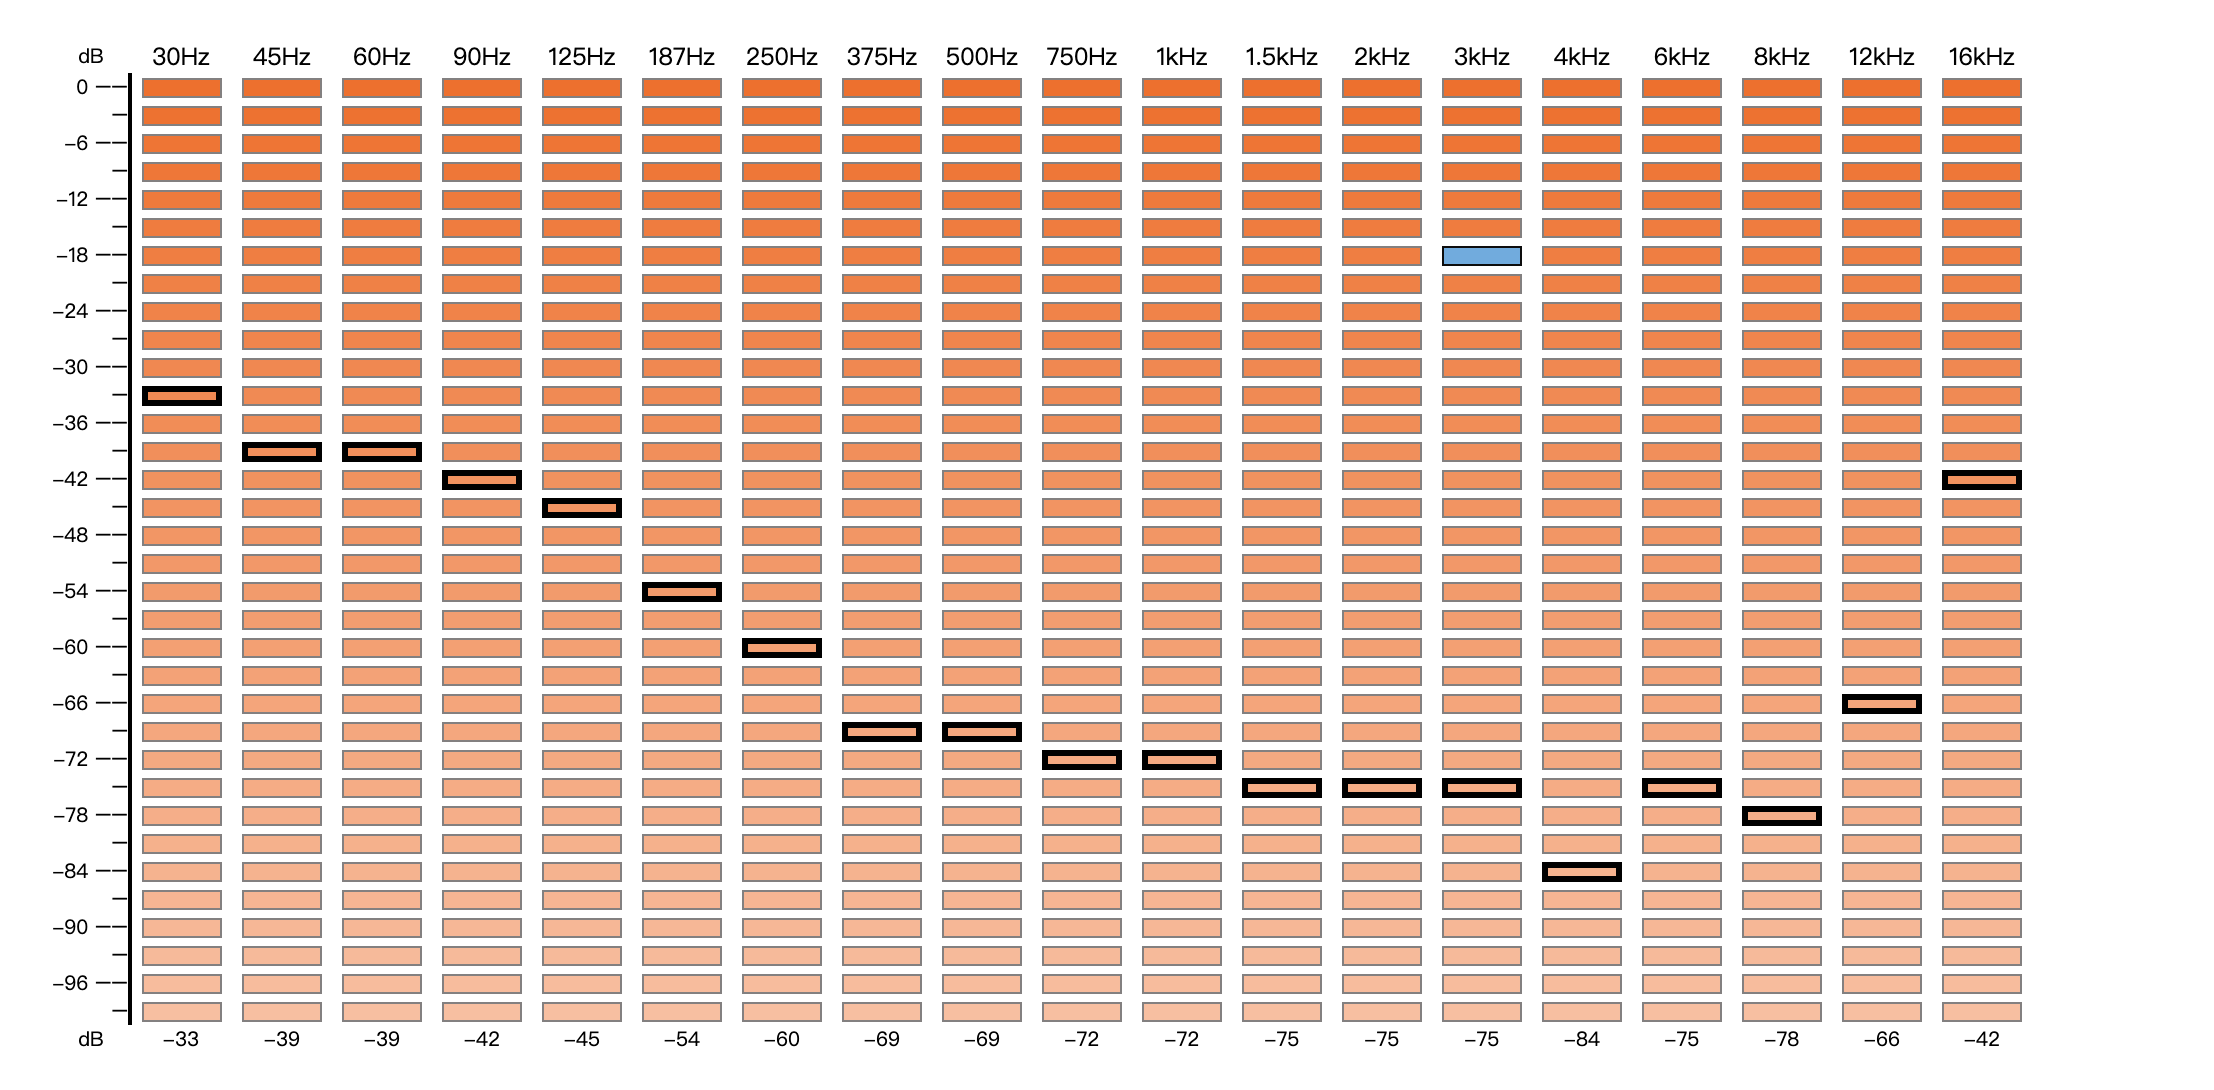
\includegraphics[width=0.95\textwidth]{figures/sensitivity.png}
    \caption{Problem 2 在线听觉测试结果（最小声音敏感度曲线）}
\end{figure}

\subsection{结论}
等响度曲线整体呈典型 U 形：约 \SIrange{1}{2}{kHz} 附近所需声压级最低，向低频端（\SIrange{30}{125}{Hz}）和高频端（\SIrange{8}{16}{kHz}）逐步升高。该趋势说明在主观响度匹配条件下，中频段具有更高的听觉效率，而低频和高频需要更高声压级才能达到相近的感知响度。

最小声音敏感度（听阈）曲线进一步给出了“刚可听见”条件下的频率依赖特性。实验结果显示，听阈在中频段（约 4kHz）达到最低，低频与高频区域听阈显著抬升，反映出人耳对中频信息的天然敏感性以及对两端频带较弱的检测能力。综合两类曲线可见，本次在线测试结果与经典听觉特性一致，为后续语音增强与感知评价中采用频率加权分析提供了实验依据。

\section{Problem 3：噪声语音构造与时频分析}

\subsection{题目要求逐条对应}
\begin{table}[H]
\centering
\begin{tabular}{>{\centering\arraybackslash}p{1.3cm}p{9.8cm}p{3.2cm}}
\toprule
要求编号 & 题目要求 & 本文对应位置 \\
\midrule
1 & 对 \texttt{mhint\_01\_01.wav} 添加白噪声，SNR=5 dB 与 0 dB & \S3.2 \\
2 & 将带噪语音能量归一化到干净语音能量 & \S3.2 \\
3 & 绘制 clean 与 equalized noisy 的波形和频谱 & \S3.3 \\
4 & 绘制 clean 与 noisy（5/0 dB）的语谱图 & \S3.4 \\
\bottomrule
\end{tabular}
\end{table}

\subsection{加噪与能量归一化}
对 clean speech 分别生成 5 dB 与 0 dB 白噪语音，随后执行
\(y_{eq}=y/\|y\|\cdot\|clean\|\) 做能量均衡。实测 SNR 与目标值一致（约 5 dB 和 0 dB）。

\subsection{波形与频谱结果}
\begin{figure}[H]
    \centering
    
\includegraphics[width=0.9\textwidth]{figures/fig04.png}
    \caption{Problem 3 波形：clean 与 equalized noisy（5 dB/0 dB）}
\end{figure}

\begin{figure}[H]
    \centering
    
\includegraphics[width=0.9\textwidth]{figures/fig05.png}
    \caption{Problem 3 频谱：clean、equalized noisy 5 dB、equalized noisy 0 dB（分开显示）}
\end{figure}

\subsection{语谱图结果}
\begin{figure}[H]
    \centering
    
\includegraphics[width=0.9\textwidth]{figures/fig06.png}
    \caption{Problem 3 语谱图：clean、equalized noisy 5 dB、equalized noisy 0 dB}
\end{figure}

\subsection{结果分析}
\textbf{时域层面：}在 5 dB 与 0 dB 条件下，加入白噪声后波形瞬时振幅方差明显增大；能量均衡步骤保证了不同条件下总体能量与 clean speech 可比，从而避免“仅因响度差异”带来的主观偏差。0 dB 条件下噪声与语音能量同量级，时域波形呈现明显随机起伏，但语音包络仍可辨认。

\textbf{频域层面：}与 clean speech 相比，noisy speech 的频谱噪声底整体抬升，且 0 dB 情况下抬升幅度更大。尽管白噪声在全频段分布，语音主能量区（低频至中频）仍保留相对突出的结构，因此未出现完全淹没现象。该现象与“语音结构先验 + 人耳中频敏感性”共同作用下的可懂度保留一致。

\textbf{时频层面：}语谱图显示，随 SNR 从 5 dB 降至 0 dB，背景纹理显著增强，谐波与共振峰轨迹对比度下降，但关键时频组织结构仍连续存在。这表明在本实验条件下，噪声主要降低了可见度和清晰度，而未完全破坏语音的宏观时频组织。

\textbf{结论：}Problem 3 结果与理论预期一致：SNR 下降导致噪声底抬升与时频细节退化；能量均衡后不同噪声条件可在统一能量基准下进行有效比较。

\subsection{关键代码段}
\begin{lstlisting}[caption={Problem 3 加噪、均衡与频谱分开绘制}]
% 按目标 SNR 加白噪
[yNoisy, snrActual] = addWhiteNoiseAtSNR(clean, snrTarget);

% 能量均衡到 clean
yEq = yNoisy / (norm(yNoisy) + eps) * norm(clean);

% 频谱分开绘制（clean / 5 dB / 0 dB）
[fc, mc] = oneSidedSpectrum(clean, fs);
[f5, m5] = oneSidedSpectrum(noisyEq{1}, fs);
[f0, m0] = oneSidedSpectrum(noisyEq{2}, fs);
\end{lstlisting}

\section{Problem 4：PESQ 客观质量评价}

\subsection{题目要求逐条对应}
\begin{table}[H]
\centering
\begin{tabular}{>{\centering\arraybackslash}p{1.3cm}p{9.8cm}p{3.2cm}}
\toprule
要求编号 & 题目要求 & 本文对应位置 \\
\midrule
1 & 对 clean speech 添加白噪声（-5,-3,-1,1,3,5 dB） & \S4.2 \\
2 & 将 noisy speech 能量归一化到 clean speech & \S4.2 \\
3 & 运行 PESQ 并绘制 PESQ-SNR 曲线 & \S4.3--\S4.4 \\
\bottomrule
\end{tabular}
\end{table}

\subsection{实验设置}
在 SNR=\{-5,-3,-1,1,3,5\} dB 条件下生成带噪语音并做能量均衡。调用本地 \texttt{pesq.m} 进行评分，当前 \SI{16}{kHz}（wideband）模式下使用返回的 MOS-LQO 作为 PESQ 指标。

\subsection{PESQ 结果表（PESQ保留两位小数）}
\begin{table}[H]
\centering
\begin{tabular}{S[table-format=+2.0]S[table-format=+2.2]S[table-format=1.4]}
\toprule
{SNR\_Target\_dB} & {SNR\_Actual\_dB} & {PESQ} \\
\midrule
-5 & -5.00 & 1.0741 \\
-3 & -3.00 & 1.0821 \\
-1 & -1.00 & 1.0908 \\
 1 &  1.00 & 1.1023 \\
 3 &  3.00 & 1.1164 \\
 5 &  5.00 & 1.1346 \\
\bottomrule
\end{tabular}
\caption{Problem 4 PESQ 与 SNR 对应结果}
\end{table}

\subsection{PESQ-SNR 曲线与分析}
\begin{figure}[H]
    \centering
    
\includegraphics[width=0.72\textwidth]{figures/fig07.png}
    \caption{Problem 4 PESQ 随 SNR 变化曲线}
\end{figure}

实验结果显示，PESQ 随 SNR 提升呈严格单调增长：从 \(-5\) dB 时的 1.0741 增加到 \(5\) dB 时的 1.1346，总提升约 0.0605。若以 \SI{10}{dB} 区间平均变化估计，斜率约为 \(6.05\times10^{-3}\) PESQ/dB。该趋势说明在当前噪声模型与处理流程下，噪声强度降低能够稳定改善客观质量评价指标。

进一步观察相邻 SNR 点的增量可见，PESQ 改善在高 SNR 段略有增强，反映出当语音主结构逐步从噪声中恢复时，感知质量指标对失真下降更敏感。需要指出的是，绝对分值仍处于较低区间，表明白噪声条件下即使在 5 dB 时，语音质量仍受明显影响；该结论与 Problem 3 的时频可见度变化相互印证。

综上，Problem 4 给出的量化结果不仅验证了 “SNR 提升 \(\Rightarrow\) 质量提升” 的基本关系，也为后续比较不同降噪算法在相同 SNR 条件下的客观收益提供了基线参考。

\subsection{关键代码段}
\begin{lstlisting}[caption={Problem 4 PESQ 计算与曲线绘制}]
% 使用本地 pesq.m
addpath(fileparts(pesqFile), '-begin');
scores = pesq(char(refWav), char(degWav));

% wideband / narrowband 统一取最终 MOS-LQO
pesqVal(i) = double(scores(end));

% 绘制 PESQ-SNR 曲线
plot(snrList, pesqVal, '-o', 'LineWidth', 1.5, 'MarkerSize', 7);
\end{lstlisting}

\section{实验总结}
\subsection{总结}
本次实验已完成 Problem 1、Problem 2、Problem 3、Problem 4 的要求。结果表明：
\begin{enumerate}
    \item 元音纯音合成可稳定重建不同元音的频谱包络特征；
    \item 听觉测试曲线呈典型等响度 U 形趋势；
    \item 在 5 dB/0 dB 条件下，噪声显著影响语谱可见性，但语音结构在 0 dB 仍有一定可辨性；
    \item PESQ 评分随 SNR 提升而单调增加，验证了噪声强度与主观质量指标之间的对应关系。
\end{enumerate}

\subsection{附件说明}
本报告正文中已省略音频文件细节。实验相关音频（原始、加噪、均衡、合成）统一随作业附件提交。

\ifPDFTeX\end{CJK*}\fi
\end{document}
